\subsection{Userspace: Wayland}

\begin{frame}{Wayland overview and paradigm}
  \begin{itemize}
  \item Wayland was started in 2008 as a modern replacement for the X Window system\\
    \textit{solving issues in-depth with a clean implementation from scratch}
  \item Drastic \textbf{simplification} of the stack and paradigm shift:
    \begin{itemize}
    \item The server and compositor are \textbf{unified} as the same component
    \item \textbf{Clients} are expected to do all the rendering
    \item Buffers are \textbf{shared} between client and server, no transfers
    \item Window decorations can be added by the client or the server
    \end{itemize}
  \item Improves \textbf{security} aspects:
    \begin{itemize}
    \item Isolates the input and output of each client
    \item Only the compositor can access display buffers \textit{(and provide screenshots)}
    \item Avoids running the compositor as root (using \code{systemd-logind})
    \end{itemize}
  \item No network support (can be implemented by compositors)
  \item \textbf{Weston} is the reference \textbf{Wayland} compositor
  \end{itemize}
\end{frame}

\begin{frame}{Wayland architecture: input to display roundtrip}
  \begin{minipage}{0.49\textwidth}
    \centering
    \includegraphics[height=0.7\textheight]{slides/graphics-software-userspace-wayland/wayland-architecture-roundtrip.png}
  \end{minipage}
  \hfill
  \begin{minipage}{0.49\textwidth}
    \begin{enumerate}
    \item An input event is read from the kernel by the compositor
    \item The affected client is determined and receives the event
    \item The client changes something, performs rendering and notifies the compositor
    \item The compositor updates the damaged regions in the back-buffer and performs page flip
    \end{enumerate}
  \end{minipage}
\end{frame}

\begin{frame}{Wayland protocol and architecture}
  \begin{itemize}
  \item Wayland provides a client-server \textbf{low-level API}:
    \begin{itemize}
    \item Wayland \textbf{display connections} happen through local IPC
    \item Display is identified with the \code{WAYLAND_DISPLAY} \textbf{environment variable}
    \item \textbf{Asynchronous} and \textbf{object-oriented} protocol
    \item \textbf{Objects} represent \textbf{resources} from the compositor
    \item Objects implement specific \textbf{interfaces}, with requests and events
      \begin{itemize}
      \item \textbf{Requests} are messages sent by the client, 
      \item \textbf{Events} are messages received from the server\\
        \textit{errors are only specific types of events}
      \end{itemize}
    \end{itemize}
  \item Some \textbf{implementation} details:
    \begin{itemize}
    \item IPC is a regular UNIX socket (allows passing file descriptors for zero-copy)
    \item A proxy provides client-side object representations and message translation
    \item Messages are serialized (marshalling) to the wire format
    \item Messages are buffered and flushed/dispatched when asked
    \end{itemize}
  \item Client-server protocol is implemented in \textbf{libwayland-client} and \textbf{libwayland-server}
  \item These libraries do not provide any interface implementation
  \end{itemize}
\end{frame}

\begin{frame}{Wayland core protocol: global object interfaces}
  \begin{itemize}
  \item \textbf{Global} core object interfaces:
    \begin{itemize}
    \item \code{wl_display}: manages server connection, exposes the registry
    \item \code{wl_registry}: exposes available global object interfaces
    \item \code{wl_output}: describes the output properties (mode, geometry)
    \item \code{wl_seat}: exposes input device object capabilities and interfaces
    \item \code{wl_compositor}: provides surfaces and regions for composition
    \item \code{wl_subcompositor}: provides sub-surfaces for in-surface compositing
    \item \code{wl_shm}: exposes a shared memory interface
    \item \code{wl_data_device_manager}: support for copy/paste between clients
    \end{itemize}
  \item Global object interfaces are bound with the registry before use
    \begin{itemize}
    \item Using global \code{struct wl_interface} definitions
    \item \code{wl_registry_bind} returns a pointer to a proxy object
    \end{itemize}
  \item Global objects give access to other \textbf{specific objects}
  \end{itemize}
\end{frame}

\begin{frame}{Wayland core protocol: specific object interfaces}
  \begin{itemize}
  \item \textbf{Input-related} (\code{wl_seat}) specific core object interfaces:
    \begin{itemize}
    \item \code{wl_pointer}: exposes mice events and cursor
    \item \code{wl_keyboard}: exposes keyboard events and information
    \item \code{wl_touch}: exposes touchscreen events
    \end{itemize}
  \item \textbf{Compositor-related} (\code{wl_compositor}) specific core object interfaces:
    \begin{itemize}
    \item \code{wl_region}: specifies any area
    \item \code{wl_surface}: rectangular on-screen pixel area
      \begin{itemize}
      \item contents set to a \code{wl_buffer} (can be transformed)
      \item configured with a \code{wl_region} for input
      \item configured with a \code{wl_region} for area-based opacity
      \item updated with buffer damage regions
      \end{itemize}
    \item \code{wl_subsurface}: converts \code{wl_surface} objects to positioned sub-surfaces
    \end{itemize}
  \item \textbf{Shared memory-related} (\code{wl_shm}) specific core object interfaces:
    \begin{itemize}
    \item \code{wl_shm_pool}: allows creating shared-memory buffers
    \end{itemize}
  \item \textbf{Memory-related} specific core object interfaces:
    \begin{itemize}
    \item \code{wl_buffer}: generic object for a \code{wl_surface}
    \end{itemize}
  \end{itemize}
\end{frame}

\begin{frame}{Wayland extra protocols}
  \begin{itemize}
  \item Extra protocols (object interfaces) can be \textbf{exposed by the compositor}
    \begin{itemize}
    \item Protocols (including the core) are described as XML files
    \item The \code{wayland-scanner} tool produces client and server C code and headers
    \item Accepted additional protocol descriptions are available at:
      \url{https://gitlab.freedesktop.org/wayland/wayland-protocols}
    \item Some are considered stable and many unstable
    \end{itemize}
  \item Some widely-used \textbf{protocol extensions}:
    \begin{itemize}
    \item \textbf{XDG-Shell}: desktop shell integration
      \begin{itemize}
      \item Turns \code{wl_surfaces} to \code{xdg_surfaces} that can be resized, minimized, etc
      \item Provides a popup/menu interface with \code{xdg_popup}
      \end{itemize}
    \item \textbf{IVI-Shell}: In-vehicle shell with surface layers
    \item \textbf{Presentation time}: Precise timing and event feedback
    \end{itemize}
  \end{itemize}
\end{frame}

\begin{frame}{Wayland OpenGL integration}
  \begin{itemize}
    \item Wayland supports EGL for windowing integration with OpenGL
    \item \code{eglGetDisplay} is called with a \code{struct wl_display}\\
      \textit{mesa's \code{_eglNativePlatformDetectNativeDisplay} figures it out}
    \item Mesa 3D implements Wayland EGL interface for OpenGL integration
      \begin{itemize}
      \item Needs to implement DRI2 for DRM authentication
      \item \code{wl_drm} interface between the wayland EGL client and the compositor
      \item Both sides are actually implemented in mesa
      \item The interface is bound to the compositor with \code{eglBindWaylandDisplayWL}\\
        \textit{using the compositor's EGL context as entry-point to mesa}
      \item Allows sharing DRM GEM buffers with the compositor
      \end{itemize}
    \item Regular \code{wl_surfaces} can be bound to EGL:
      \begin{itemize}
      \item Converted to a \code{wl_egl_window} with \code{wl_egl_window_create}
      \item Then converted to an \code{EGLSurface} with \code{eglCreateWindowSurface}
      \end{itemize}
    \end{itemize}
\end{frame}

\begin{frame}{Wayland OpenGL integration (illustrated)}
  \begin{center}
  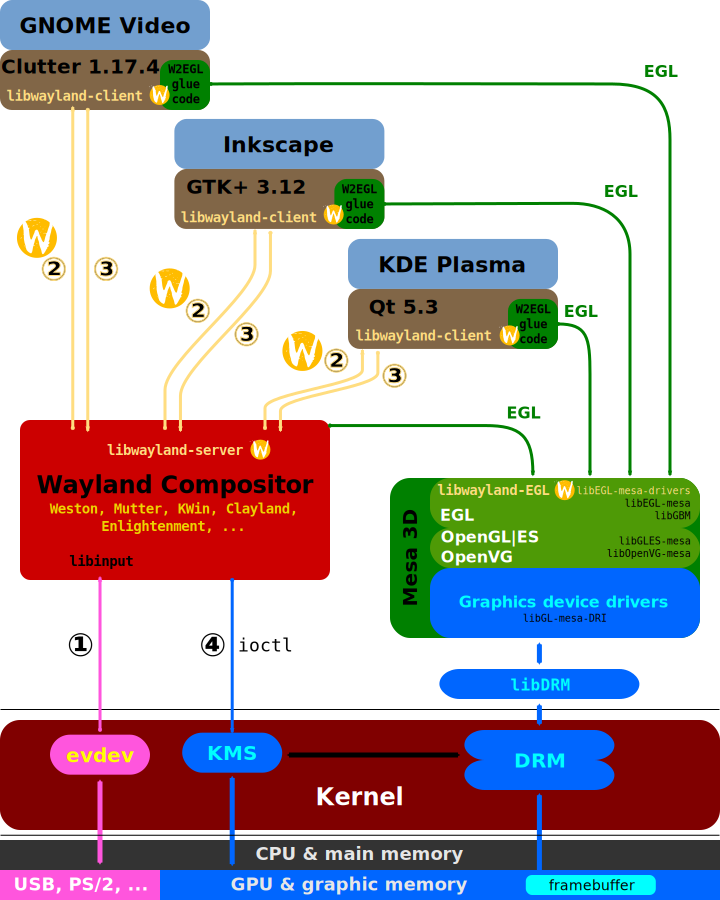
\includegraphics[width=12em]{slides/graphics-software-userspace-wayland/wayland-egl.pdf}\\
  \textit{\small Wayland integration with EGL}\\
  \end{center}
\end{frame}

\begin{frame}{Wayland status and adoption}
  \begin{itemize}
  \item Wayland is now quite mature, robust, efficient and widely used
    \begin{itemize}
    \item Most toolkits have support for it: GTK 3, Qt 5, SDL, EFL
    \item Major desktop environments support it: GNOME 3, KDE Plasma 5
    \item Integrated sessions with login managers from \code{/usr/share/wayland-sessions}
    \item Runs with user privileges with \code{systemd-logind}
    \end{itemize}
  \item X11 applications can be integrated using \textbf{XWayland}
    \begin{itemize}
    \item X server implementation registered as a Wayland client
    \item Wayland composer acts as X compositing window manager
    \item Creates a \code{wl_surface} for each window, redirects input/output
    \end{itemize}
  \item Diverse compositor implementations have emerged
    \begin{itemize}
    \item Sometimes tied to a desktop environment: mutter, kwin
    \item \textbf{libinput} was created to help with input aspects
    \item \textbf{libweston} emerged from the \textbf{Weston} compositor core
    \item \textbf{wlroots} emerged from the \textbf{Sway} compositor core
    \item Support \textbf{DRM KMS} display, \textbf{EGL} rendering (\textbf{pixman} supported by libweston)
    \end{itemize}
  \end{itemize}
\end{frame}

\begin{frame}{Wayland stack overview (illustrated)}
  \begin{center}
  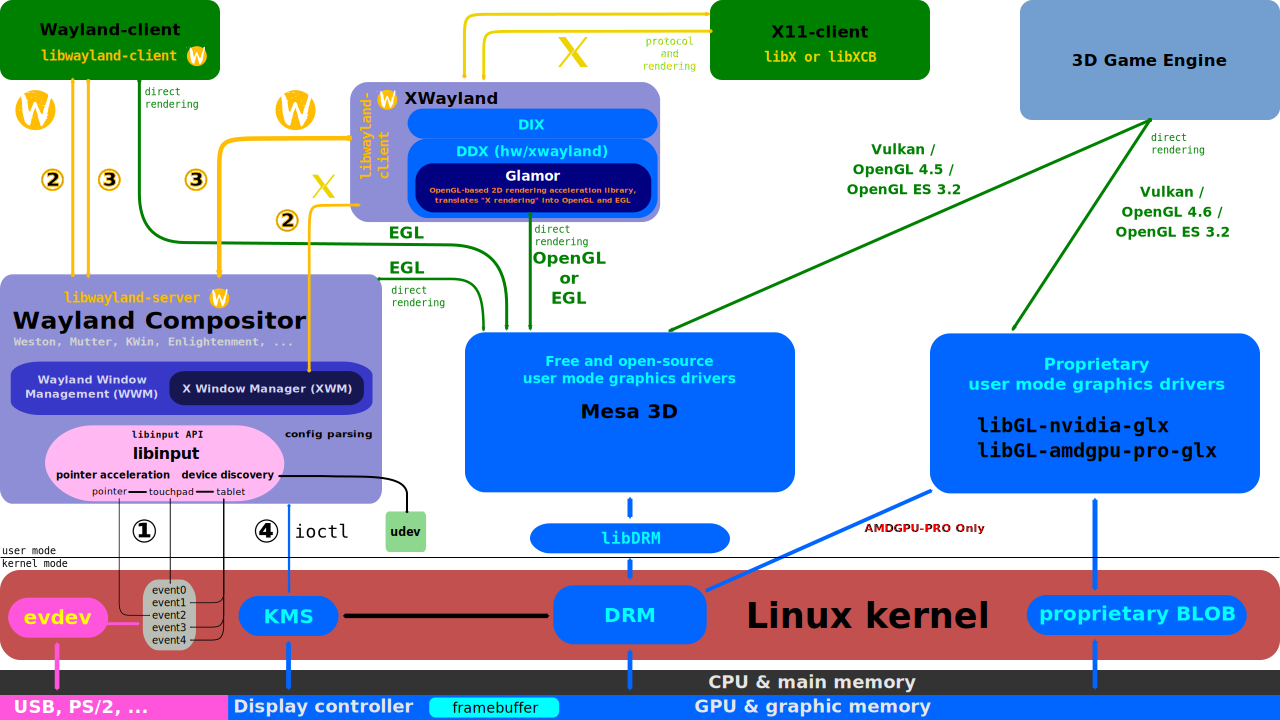
\includegraphics[width=0.8\textwidth]{slides/graphics-software-userspace-wayland/wayland-stack.pdf}\\
  \textit{\small The graphics stack with Wayland}\\
  \end{center}
\end{frame}

\begin{frame}[fragile]{Wayland debug and documentation}
  \begin{itemize}
  \item \textbf{Debugging} tips:
    \begin{itemize}
    \item Supported global object interfaces can be listed with \code{weston-info}
    \item The \code{WAYLAND_DEBUG} environment variable enables protocol tracing
    \end{itemize}
  \item \textbf{Weston debugging}:
    \begin{itemize}
    \item Debug arguments: \code{--debug}, \code{--log=file.log}
    \item Grabbing a different TTY argument: \code{--tty 1}
    \item Wireframe keystroke: \code{mod + shift + space + F}
    \item Timeline recording (to a JSON file) keystroke: \code{mod + shift + space + d}\\
      \textit{can produce a graph with \url{https://github.com/ppaalanen/wesgr}}
    \end{itemize}
  \item \textbf{Community} contact:
    \begin{itemize}
    \item Mailing list: \code{wayland-devel@lists.freedesktop.org}
    \item IRC channel: \code{#wayland} on the OFTC network
    \end{itemize}
  \item \textbf{Documentation} resources:
    \begin{itemize}
    \item Online wiki of the project: \url{https://wayland.freedesktop.org/}
    \item Online documentation: \url{https://wayland.freedesktop.org/docs/html/}
    \end{itemize}
  \end{itemize}
\end{frame}
